\documentclass{standalone}
\usepackage{tikz}
\usetikzlibrary{patterns, positioning}


\begin{document}
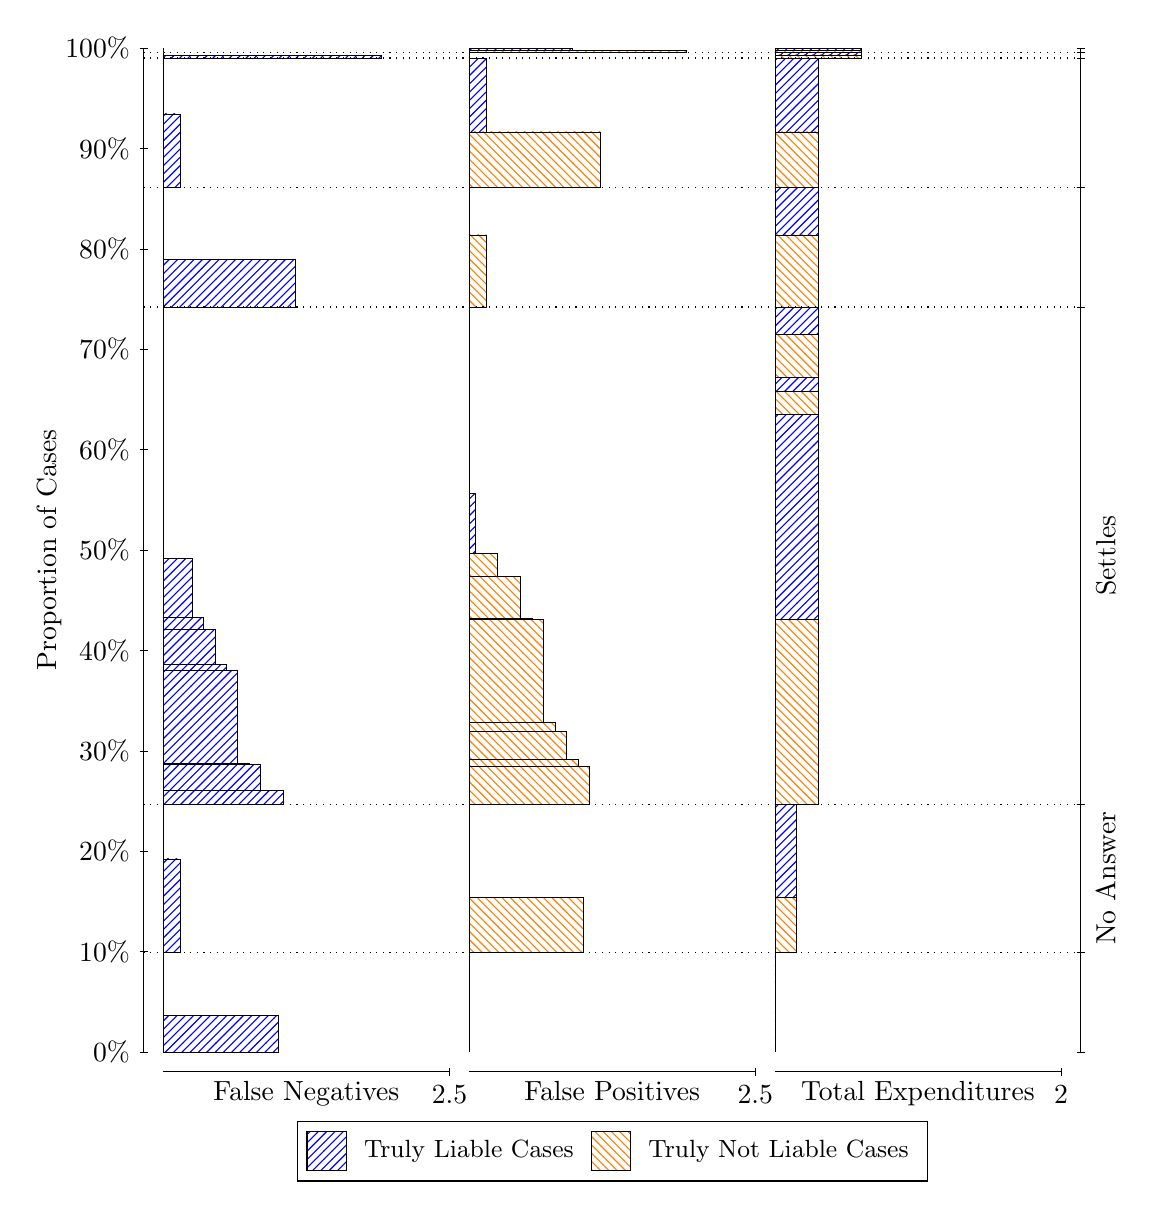
\begin{tikzpicture}
\draw[black, very thin] (1.5,1.75) -- (1.5,14.5);
\node[rotate=90, text=black, anchor=center] at (0.3, 8.125) {Proportion of Cases};
\draw[black, very thin] (1.45,1.75) -- (1.55,1.75);
\node[text=black, anchor=east] at (1.45, 1.75) {0\%};
\draw[black, very thin] (1.45,3.025) -- (1.55,3.025);
\node[text=black, anchor=east] at (1.45, 3.025) {10\%};
\draw[black, very thin] (1.45,4.3) -- (1.55,4.3);
\node[text=black, anchor=east] at (1.45, 4.3) {20\%};
\draw[black, very thin] (1.45,5.575) -- (1.55,5.575);
\node[text=black, anchor=east] at (1.45, 5.575) {30\%};
\draw[black, very thin] (1.45,6.85) -- (1.55,6.85);
\node[text=black, anchor=east] at (1.45, 6.85) {40\%};
\draw[black, very thin] (1.45,8.125) -- (1.55,8.125);
\node[text=black, anchor=east] at (1.45, 8.125) {50\%};
\draw[black, very thin] (1.45,9.4) -- (1.55,9.4);
\node[text=black, anchor=east] at (1.45, 9.4) {60\%};
\draw[black, very thin] (1.45,10.675) -- (1.55,10.675);
\node[text=black, anchor=east] at (1.45, 10.675) {70\%};
\draw[black, very thin] (1.45,11.95) -- (1.55,11.95);
\node[text=black, anchor=east] at (1.45, 11.95) {80\%};
\draw[black, very thin] (1.45,13.225) -- (1.55,13.225);
\node[text=black, anchor=east] at (1.45, 13.225) {90\%};
\draw[black, very thin] (1.45,14.5) -- (1.55,14.5);
\node[text=black, anchor=east] at (1.45, 14.5) {100\%};

\draw[black, very thin] (13.4,1.75) -- (13.4,14.5);
\draw[black, very thin] (13.35,1.75) -- (13.45,1.75);
\node[anchor=west] at (13.35, 1.75) {};
\draw[black, very thin] (13.35,3.0166) -- (13.45,3.0166);
\node[anchor=west] at (13.35, 3.0166) {};
\draw[black, very thin] (13.35,4.8945) -- (13.45,4.8945);
\node[anchor=west] at (13.35, 4.8945) {};
\draw[black, very thin] (13.35,11.211) -- (13.45,11.211);
\node[anchor=west] at (13.35, 11.211) {};
\draw[black, very thin] (13.35,12.727) -- (13.45,12.727);
\node[anchor=west] at (13.35, 12.727) {};
\draw[black, very thin] (13.35,14.373) -- (13.45,14.373);
\node[anchor=west] at (13.35, 14.373) {};
\draw[black, very thin] (13.35,14.445) -- (13.45,14.445);
\node[anchor=west] at (13.35, 14.445) {};
\draw[black, very thin] (13.35,14.5) -- (13.45,14.5);
\node[anchor=west] at (13.35, 14.5) {};

\draw[black, very thin, pattern color=blue, pattern=north east lines] (1.75,1.75) rectangle (3.2033,2.2182);
\draw[black, very thin, pattern color=orange, pattern=north west lines] (1.75,2.2182) rectangle (1.75,3.0166);
\draw[black, very thin, pattern color=blue, pattern=north east lines] (1.75,3.0166) rectangle (1.968,4.2012);
\draw[black, very thin, pattern color=orange, pattern=north west lines] (1.75,4.2012) rectangle (1.75,4.8945);
\draw[black, very thin, pattern color=blue, pattern=north east lines] (1.75,4.8945) rectangle (3.276,5.073);
\draw[black, very thin, pattern color=blue, pattern=north east lines] (1.75,5.073) rectangle (2.9853,5.4023);
\draw[black, very thin, pattern color=blue, pattern=north east lines] (1.75,5.4023) rectangle (2.84,5.4158);
\draw[black, very thin, pattern color=blue, pattern=north east lines] (1.75,5.4158) rectangle (2.6947,6.5959);
\draw[black, very thin, pattern color=blue, pattern=north east lines] (1.75,6.5959) rectangle (2.5493,6.6753);
\draw[black, very thin, pattern color=blue, pattern=north east lines] (1.75,6.6753) rectangle (2.404,7.1177);
\draw[black, very thin, pattern color=blue, pattern=north east lines] (1.75,7.1177) rectangle (2.2587,7.2645);
\draw[black, very thin, pattern color=blue, pattern=north east lines] (1.75,7.2645) rectangle (2.1133,8.0188);
\draw[black, very thin, pattern color=orange, pattern=north west lines] (1.75,8.0188) rectangle (1.75,11.211);
\draw[black, very thin, pattern color=blue, pattern=north east lines] (1.75,11.211) rectangle (3.4213,11.811);
\draw[black, very thin, pattern color=orange, pattern=north west lines] (1.75,11.811) rectangle (1.75,12.727);
\draw[black, very thin, pattern color=blue, pattern=north east lines] (1.75,12.727) rectangle (1.968,13.665);
\draw[black, very thin, pattern color=orange, pattern=north west lines] (1.75,13.665) rectangle (1.75,14.373);
\draw[black, very thin, pattern color=blue, pattern=north east lines] (1.75,14.373) rectangle (4.5113,14.404);
\draw[black, very thin, pattern color=orange, pattern=north west lines] (1.75,14.404) rectangle (1.75,14.445);
\draw[black, very thin, pattern color=orange, pattern=north west lines] (1.75,14.445) rectangle (1.75,14.47);
\draw[black, very thin, pattern color=blue, pattern=north east lines] (1.75,14.47) rectangle (1.75,14.5);
\draw[black, very thin, pattern color=orange, pattern=north west lines] (5.6333,1.75) rectangle (5.6333,2.5484);
\draw[black, very thin, pattern color=blue, pattern=north east lines] (5.6333,2.5484) rectangle (5.6333,3.0166);
\draw[black, very thin, pattern color=orange, pattern=north west lines] (5.6333,3.0166) rectangle (7.0867,3.71);
\draw[black, very thin, pattern color=blue, pattern=north east lines] (5.6333,3.71) rectangle (5.6333,4.8945);
\draw[black, very thin, pattern color=orange, pattern=north west lines] (5.6333,4.8945) rectangle (7.1593,5.3799);
\draw[black, very thin, pattern color=orange, pattern=north west lines] (5.6333,5.3799) rectangle (7.014,5.4634);
\draw[black, very thin, pattern color=orange, pattern=north west lines] (5.6333,5.4634) rectangle (6.8687,5.8222);
\draw[black, very thin, pattern color=orange, pattern=north west lines] (5.6333,5.8222) rectangle (6.7233,5.9309);
\draw[black, very thin, pattern color=orange, pattern=north west lines] (5.6333,5.9309) rectangle (6.578,7.2436);
\draw[black, very thin, pattern color=orange, pattern=north west lines] (5.6333,7.2436) rectangle (6.4327,7.2581);
\draw[black, very thin, pattern color=orange, pattern=north west lines] (5.6333,7.2581) rectangle (6.2873,7.7902);
\draw[black, very thin, pattern color=orange, pattern=north west lines] (5.6333,7.7902) rectangle (5.9967,8.0866);
\draw[black, very thin, pattern color=blue, pattern=north east lines] (5.6333,8.0866) rectangle (5.706,8.8408);
\draw[black, very thin, pattern color=blue, pattern=north east lines] (5.6333,8.8408) rectangle (5.6333,11.211);
\draw[black, very thin, pattern color=orange, pattern=north west lines] (5.6333,11.211) rectangle (5.8513,12.127);
\draw[black, very thin, pattern color=blue, pattern=north east lines] (5.6333,12.127) rectangle (5.6333,12.727);
\draw[black, very thin, pattern color=orange, pattern=north west lines] (5.6333,12.727) rectangle (7.3047,13.435);
\draw[black, very thin, pattern color=blue, pattern=north east lines] (5.6333,13.435) rectangle (5.8513,14.373);
\draw[black, very thin, pattern color=orange, pattern=north west lines] (5.6333,14.373) rectangle (5.6333,14.414);
\draw[black, very thin, pattern color=blue, pattern=north east lines] (5.6333,14.414) rectangle (5.6333,14.445);
\draw[black, very thin, pattern color=orange, pattern=north west lines] (5.6333,14.445) rectangle (8.3947,14.47);
\draw[black, very thin, pattern color=blue, pattern=north east lines] (5.6333,14.47) rectangle (6.9413,14.5);
\draw[black, very thin, pattern color=orange, pattern=north west lines] (9.5167,1.75) rectangle (9.5167,2.5484);
\draw[black, very thin, pattern color=blue, pattern=north east lines] (9.5167,2.5484) rectangle (9.5167,3.0166);
\draw[black, very thin, pattern color=orange, pattern=north west lines] (9.5167,3.0166) rectangle (9.7892,3.71);
\draw[black, very thin, pattern color=blue, pattern=north east lines] (9.5167,3.71) rectangle (9.7892,4.8945);
\draw[black, very thin, pattern color=orange, pattern=north west lines] (9.5167,4.8945) rectangle (10.062,7.2436);
\draw[black, very thin, pattern color=blue, pattern=north east lines] (9.5167,7.2436) rectangle (10.062,9.8466);
\draw[black, very thin, pattern color=orange, pattern=north west lines] (9.5167,9.8466) rectangle (10.062,10.143);
\draw[black, very thin, pattern color=blue, pattern=north east lines] (9.5167,10.143) rectangle (10.062,10.321);
\draw[black, very thin, pattern color=orange, pattern=north west lines] (9.5167,10.321) rectangle (10.062,10.868);
\draw[black, very thin, pattern color=blue, pattern=north east lines] (9.5167,10.868) rectangle (10.062,11.211);
\draw[black, very thin, pattern color=orange, pattern=north west lines] (9.5167,11.211) rectangle (10.062,12.127);
\draw[black, very thin, pattern color=blue, pattern=north east lines] (9.5167,12.127) rectangle (10.062,12.727);
\draw[black, very thin, pattern color=orange, pattern=north west lines] (9.5167,12.727) rectangle (10.062,13.435);
\draw[black, very thin, pattern color=blue, pattern=north east lines] (9.5167,13.435) rectangle (10.062,14.373);
\draw[black, very thin, pattern color=orange, pattern=north west lines] (9.5167,14.373) rectangle (10.607,14.414);
\draw[black, very thin, pattern color=blue, pattern=north east lines] (9.5167,14.414) rectangle (10.607,14.445);
\draw[black, very thin, pattern color=orange, pattern=north west lines] (9.5167,14.445) rectangle (10.607,14.47);
\draw[black, very thin, pattern color=blue, pattern=north east lines] (9.5167,14.47) rectangle (10.607,14.5);
\draw[black, dotted] (1.5,3.0166) -- (13.4,3.0166);
\draw[black, dotted] (1.5,4.8945) -- (13.4,4.8945);
\draw[black, dotted] (1.5,11.211) -- (13.4,11.211);
\draw[black, dotted] (1.5,12.727) -- (13.4,12.727);
\draw[black, dotted] (1.5,14.373) -- (13.4,14.373);
\draw[black, dotted] (1.5,14.445) -- (13.4,14.445);
\draw[black, very thin] (1.75,1.5) -- (5.3833,1.5);
\node[text=black, anchor=north] at (3.5667, 1.5) {False Negatives};
\draw[black, very thin] (5.3833,1.45) -- (5.3833,1.55);
\node[text=black, anchor=north] at (5.3833, 1.45) {2.5};

\draw[black, very thin] (5.6333,1.5) -- (9.2667,1.5);
\node[text=black, anchor=north] at (7.45, 1.5) {False Positives};
\draw[black, very thin] (9.2667,1.45) -- (9.2667,1.55);
\node[text=black, anchor=north] at (9.2667, 1.45) {2.5};

\draw[black, very thin] (9.5167,1.5) -- (13.15,1.5);
\node[text=black, anchor=north] at (11.333, 1.5) {Total Expenditures};
\draw[black, very thin] (13.15,1.45) -- (13.15,1.55);
\node[text=black, anchor=north] at (13.15, 1.45) {2};


\node[text=black, centered, rotate=90] at (13.72, 3.9556) {No Answer};
\node[text=black, centered, rotate=90] at (13.72, 8.0527) {Settles};





\draw (7.449999999999999,1.5) node[draw=none] (baseCoordinate) {};
\begin{scope}[align=center]
        \matrix[scale=0.5, draw=black, below=0.5cm of baseCoordinate, nodes={draw}, column sep=0.1cm]{
            \node[rectangle, draw, minimum width=0.5cm, minimum height=0.5cm, pattern color=blue, pattern=north east lines] {}; &
            \node[draw=none, font=\small, text=black] (B) {Truly Liable Cases}; &
            \node[rectangle, draw, minimum width=0.5cm, minimum height=0.5cm, pattern color=orange, pattern=north west lines] {}; &
            \node[draw=none, font=\small, text=black] (B) {Truly Not Liable Cases}; \\
            };
\end{scope}

\end{tikzpicture}
\end{document}